% Local IspellDict: english

\documentclass[a4paper,12pt,twoside]{article}
\usepackage[english]{babel}
\usepackage{graphicx}
\usepackage{listings}

\lstset{
	language=ada,
	basicstyle=\footnotesize,
	numbers=left,
	numberstyle=\footnotesize,
	stepnumber=2,
	numbersep=5pt,
	showspaces=false,
	showstringspaces=false,
	showtabs=false,
	tabsize=2,
	captionpos=b,
	breaklines=true,
	breakatwhitespace=false
}
	
\widowpenalty=10000
\clubpenalty=10000

\begin{document}
\noindent\parbox[t]{9cm}{\textsf{Course 02158 Concurrent Programming\\
Fall 2011, DTU Informatics }}
\hfill
\parbox[t]{1cm}{\mbox{}\\
\raisebox{0.0cm}[1cm][1cm]{
\includegraphics[origin=lb]{dtu_logo_cmyk.pdf}}}

\vspace{2cm}

\begin{center}
{\Large \bf Solution to the mandatory assignment}\\
\vspace{0.3cm}
{\it Due Date : 16/11/2011}\\
\vspace{1cm}
{\Large Group 19}\\
\vspace{0.3cm}
\begin{tabular}{ccc}
{\large Jakub Judas}&{\large Nicolas Silva}&{\large Robin Del\'earde}\\
s110845&s111781&s111873
\end{tabular}\\
\end{center}

\newpage

\section{Introduction: the cars control problem}




\section{Step 3: the Barrier}

The purpose of this step is to implement a barrier on the playground in order to prevent the cars from making more rounds than the others. This is done by making every car stop at a barrier line, and wait for all the others before starting a new round. This synchronization issue can be solved with semaphores, which make it possible to check if all the cars are present at the barrier, and to make them wait while that's not the case, since a car is nothing more than a thread.

\begin{figure}[h]
   \caption{\label{Barrier} crossing the barrier}
   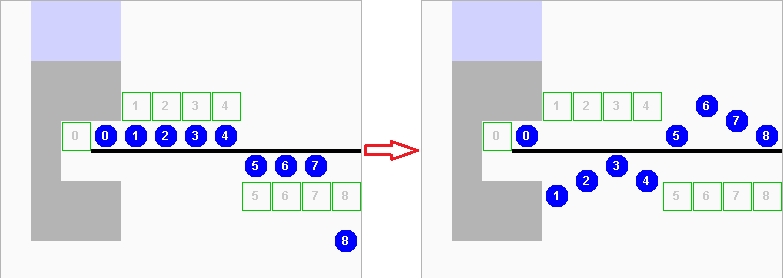
\includegraphics[width=14cm]{screens/Barrier}
\end{figure}

\subsection{Our solution: a counter and a table of 9 semaphores}
In order to stop those Car-threads, each car is assigned a semaphore, whose value is 0 while the car is not allowed to pass the barrier (the starting value is 0), and 1 either, thanks to a V operation triggered by the last car awaited. Those 9 semaphores are stored in a table called \textbf{barrier}.\\

\noindent A barrier is defined by the Barrier class as:\\
 - a table of 9 semaphores as described previously;\\
 - a boolean \textbf{ison} to control the state of the barrier;\\
 - an integer \textbf{count} responsible for counting the number of cars waiting at the barrier;\\
 - another boolean \textbf{pass}, whose role is to allow a car to pass the barrier or not. The value of it is changed by the penultimate car reaching the barrier, so as to allow the last car on the playground to know it, and to release all the others when reaching the barrier.\\

The access control at the barrier is done in the method \textit{sync}, whose code is given below (\textbf{no} is the number of the car reaching this step):
\begin{verbatim}
public Barrier() {
	pass = false;
	count = 0;
	barrier = new Semaphore[9];
	for (int i=0; i<9; i++) {
		barrier[i] = new Semaphore(0);
	}
}
		
public void sync(int no) {
   if (!pass) {
	   count++;
	   //the penultimate car gives access to the last one
	   if (count==8) {
		   pass = true;
	   }
	   //the cars are stopped by the barrier
	   try  {barrier[no].P();} catch (InterruptedException e) {}
   }
   //the last car may pass here and releases everyone
   else {
	   pass = false;
	   count = 0;
	   for (int i=0; i<9; i++) {
		   if (i!=no) {
			   barrier[i].V();
		   }
	   }
   }
}
\end{verbatim}

\subsection{A first attempt with semaphores only}
Using semaphores in this step, the temptation is to use them both to count the cars at the barrier and to stop them. However a single semaphore initialized to a positive value allows a thread to execute, whereas we want to stop the cars while they are not 9. Hence a first idea was to use a semaphore to count the cars reaching the barrier, and another one to stop them if there are still cars running. The first semaphore was initialized to 7 and its role was to enable only 7 cars to reach the stopping semaphore. Then it stopped the 8th one, and a boolean was used to determine if a car was the last one or not. As in the final solution, the last one was then accessing a part of code devoted to release everyone. This gives the following code:

\begin{verbatim}
public Barrier() {
	pass = false;
	access = new Semaphore(0);
	barrier = new Semaphore[9];
	for (int i=0; i<9; i++) {
		barrier[i] = new Semaphore(0);
	}
}

public void sync(int no) {
   if (!pass) {
	   pass = true;
	   //only 7 cars may access this zone, the 8th one is stopped here
	   try {access.P();} catch (InterruptedException e) {}
	   pass = false;
	   //the cars are stopped by the barrier
	   try {barrier[no].P();} catch (InterruptedException e) {}
   }
   //the last car may pass here and releases everyone
   else {
	   pass = false;
	   for (int i=0; i<9; i++) {
		   if (i!=no) {
			   access.V();
			   barrier[i].V();
		   }
	   }
   }
}
\end{verbatim}

\noindent The problem with this solution is due to the test done at the beginning: in fact in the case of two cars arriving at nearly the same moment, the first one can set the boolean \textbf{pass} to true, and in that way enable the second one to pass the barrier, reaching the part of the code normally dedicated to the last car. And this atomicity problem couldn't be solved by setting a semaphore as for the alley for instance, because it would have blocked all the cars.\\
%make an example with a test on the GUI
Actually the solution with an integer instead of a semaphore to count the cars is more simplistic, and doesn't even face those atomicity problems, as we proved with \textbf{spin}.

\subsection{Results of the testing with spin (extra (B))}


\subsection{Controlling the barrier (with extra (C))}
Another thing asked in this step was to make it possible to activate and deactivate the barrier by pressing buttons on the GUI. This is done by changing the value of a boolean, and reinitialize the barrier object every time it is asked: the method \textit{off} releases all the cars awaiting at the barrier, and the method \textit{on} creates a new barrier with the initialization parameters.\\

\noindent A last method called \textit{shutDown} makes it possible to deactivate the barrier only when all the cars have made the same number of rounds since it was activated, that's to say after every car has finished its current round.\\
The solution used to achieve that is to synchronize the deactivation of the barrier with one of the cars: the shut-down operation is stopped as if the car wanted to pass two times, and is released when all the cars have arrived. However this often has to wait one round to be executed, because it depends on which car arrives first at the barrier. If that's the car chosen for the synchronization, then it doesn't have to wait, otherwise it does. That's why we choose the car no.0 to do that, since it's always the first reaching the barrier, if it's not stopped by the user.
%testing with 2 different cars

\section{Step 5: the Bridge}

The bridge constructed above the hut requires new constraints on the control of the cars. Here we have to implement a component that prevent the cars from being more numerous than a fixed limit on the bridge. Moreover, is must be possible to dynamically change the limit during the running. Once more we can use semaphores to solve this coordination problem.

\subsection{Our solution: a semaphore shared by the methods enter and leave}
The first idea is obviously to use a semaphore to allow the cars to access the bridge. Its initial value is set by the current limit. Then it must be possible to change the limit without disturbing the good running of the program, i.e. taking care of the possibility to have cars on the bridge.\\
Nevertheless it is allowed to exceed the limit for a while, when the limit is lowered whereas there are already too many cars on the bridge. So we can wait that all the cars have left the bridge to change its load limit. We had 2 possibilities for that: change the limit with the first car reaching the bridge, or with the last one leaving it. This suppose to keep the track of the numbers of cars on the bridge, allowing to set the new limit only when it's 0.\\
Our solution is similar since we keep in memory the last car entered, and set the new limit only if it's still that one when it leaves the bridge. Thus the class \textit{Bridge} contains the following:

\begin{verbatim}
public Bridge() {
	limit = 1;
	bridge = new Semaphore(limit);
	atomicAccess = new Semaphore(1);
	wSetLimit = false;
}

public void enter(int no) {
	lastEntered = no;
	try {bridge.P();} catch (InterruptedException e) {}
}

public void leave(int no) {
	bridge.V();
	try {atomicAccess.P();} catch (InterruptedException e) {}
	if (wSetLimit && no == lastEntered) {
		bridge = new Semaphore(limit);
		wSetLimit = false;
	}
	atomicAccess.V();
}

public void setLimit(int k) {
	limit = k;
	wSetLimit = true;
}
\end{verbatim}



\end{document}